\chapter{Introduzione}
Nei capitoli successivi verrà presentato il progetto realizzato per l'esame di
Machine Learning del corso di laurea magistrale in informatica dell'Università
degli Studi di Milano-Bicocca.

L'intero progetto si basa sul riconoscimento della presenza di un tumore al
cervello data l'immagine di una risonanza magnetica.


Il dataset selezionato per il presente progetto può essere ottenuto tramite il
seguente collegamento: \href{https://www.kaggle.com/datasets/jakeshbohaju/brain-tumor/data}{link}.
Esso consiste in un insieme di immagini di risonanze magnetiche del cervello
provenienti da diversi pazienti, accompagnato da un file contenente le
caratteristiche estratte da tali immagini.

Al fine di condurre il riconoscimento del tumore, sono stati utilizzati i
seguenti algoritmi:
\begin{itemize}
      \item \textbf{SVM}: è stato scelto questo modello in quanto si presta bene
            a problemi di classificazione binaria e vista la sua buona capacità
            teorica nel generalizzare.
      \item \textbf{Gaussian Naive Bayes}: è stato scelto questo modello dal
            momento che permette di modellare le probabilità esplicitamente.
      \item \textbf{Rete neurale}: è stato scelto questo modello per confrontare
            i primi due con una soluzione neurale.
\end{itemize}
Dato il contesto del problema, l'obiettivo principale sarà individuare il modello
ottimale che minimizzi i falsi negativi, mantenendo allo stesso tempo un'elevata
precisione sui veri negativi. A tale scopo, sono state condotte le seguenti
operazioni di ricerca:
\begin{itemize}
      \item \textbf{Analisi esplorativa dei dati}: studio esplorativo del dataset
            utile per effettuare le prime osservazioni sui dati.
      \item \textbf{Riduzione di dimensionalità e preprocessing del dataset}:
            applicazione di diverse trasformazioni del dataset, dalla rimozione
            dei duplicati fino alla rimozione dei valori costanti. In aggiunta è
            stata ridotta la dimensionalità utilizzando due metodi, il primo
            basato sulla rimozione delle features correlate, il secondo basato
            sull'utilizzo della Principal Component Analysis (PCA). In questa fase
            vengono quindi generati i due dataset.
      \item \textbf{Valutazione dei modelli}: per ciascun dataset si è effettuata
            una valutazione dei modelli in due passi, la prima è una valutazione
            su ciascuna effettuando un allenamento sull'$80\%$ delle istanze e
            valutando sul rimanente $20\%$, la seconda è una $10$-fold stratified
            cross-validation per una valutazione più affidabile e robusta.
            Nella prima valutazione, durante la fase di training si effettua anche
            una $5$-fold stratified cross-validation sul training set, per
            ricercare gli iperparamentri migliori da utilizzare nel modello che
            verrà successivamente valutato nelle due fasi.
      \item \textbf{Confronto tra i vari modelli}: sono stati confrontati tutti
            i modelli sia in merito ai criteri di valutazione, sia in merito ai
            tempi di apprendimento.
\end{itemize}
Sono state effettuate due validazioni a causa della dimensione del dataset,
infatti, vista la sua media dimensione si è deciso di confermare le osservazioni
indotte dalla prima valutazione effettuando una cross-validation con gli
iperparametri trovati nella fase di validazione. Nella figura \ref{fig:pipeline}
viene mostrato tutto lo schema dei passi di valutazione dei modelli.
\begin{figure}[!ht]
      \centering
      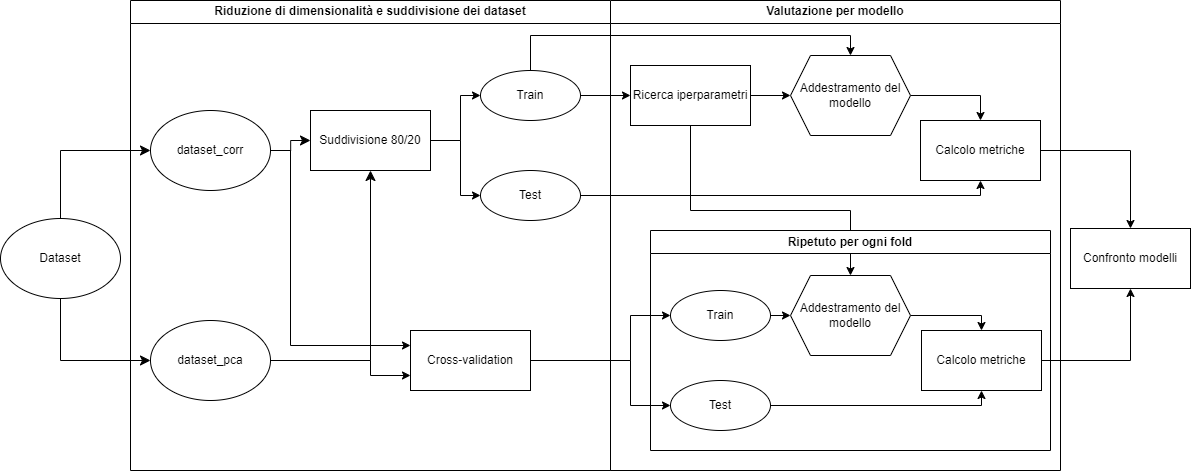
\includegraphics[width=\textwidth]{img/introduzione/schema_pipeline_valutazione_modelli.png}
      \caption{Pipeline di valutazione del singolo modello}
      \label{fig:pipeline}
\end{figure}

Per concludere, illustriamo la struttura dell'elaborato, la quale si articola
nei seguenti capitoli:
\begin{itemize}
      \item \textbf{Introduzione}: descrizione del dominio e presentazione dei
            modelli che verranno presi in considerazione per questo progetto.
      \item \textbf{Dataset}: descrizione di come è stato costruito il dataset a
            partire dalle immagini, ovvero come sono state ricavate le features,
            e relativa analisi esplorativa.
      \item \textbf{Modelli}: presentazione dei modelli e dei procedimenti svolti
            per definire i loro iperparametri.
      \item \textbf{Risultati}: presentazione dei risultati ottenuti dai modelli
            e confronto tra di essi.
      \item \textbf{Conclusioni}: conclusioni sull'elaborato.
\end{itemize}